\documentclass{article}
\usepackage{graphicx}
\usepackage{minted}


\title{SMBUD 2021 - Project work 2}
\author{\\Aman Gabba - 10793117
\\Andrea Cerasani - 10680486
\\Giovanni Demasi - 10656704
\\Pasquale Dazzeo - 10562130
\\Vlad Marian Cimpeanu - 10606922}
\date{ \begin{figure}[b] \centering 
\includegraphics[scale=0.2]{Logo Polimi.png} \end{figure}
 }
\usepackage[dvipsnames]{xcolor}

\usepackage{ifxetex}
\usepackage{ifluatex}
\newif\ifxetexorluatex % a new conditional starts as false
\ifnum 0\ifxetex 1\fi\ifluatex 1\fi>0
   \xetexorluatextrue
\fi

\ifxetexorluatex
  \usepackage{fontspec}
\else
  \usepackage[T1]{fontenc}
  \usepackage[utf8]{inputenc}
  \usepackage[lighttt]{lmodern}
\fi

\usepackage{textcomp}
\usepackage{xcolor}
\usepackage{listings}
\usepackage{upquote}

\definecolor{keyword}{HTML}{2771a3}
\definecolor{pattern}{HTML}{b53c2f}
\definecolor{string}{HTML}{be681c}
\definecolor{relation}{HTML}{7e4894}
\definecolor{variable}{HTML}{107762}
\definecolor{comment}{HTML}{8d9094}

\lstset{
	numbers=none,
	stepnumber=1,
	numbersep=5pt,
	basicstyle=\small\ttfamily,
	keywordstyle=\color{keyword}\bfseries\ttfamily,
	commentstyle=\color{comment}\ttfamily,
	stringstyle=\color{string}\ttfamily,
	identifierstyle=,
	showstringspaces=false,
	aboveskip=3pt,
	belowskip=3pt,
	columns=flexible,
	keepspaces=true,
	breaklines=true,
	captionpos=b,
	tabsize=2,
	frame=none,
}

\lstset{upquote=true}

\lstdefinelanguage{cypher}
{
	morekeywords={
		find, sort, updateMany, insertOne, countDocuments, limit
	}
}


\newcommand{\mycdots}{\cdot\!\cdot\!\cdot}
\lstset{language=cypher,
	literate=*
	{...}{$\mycdots$}{1}
	{theta}{$\theta$}{1}
}
\lstset{escapeinside={<@}{@>}}


\begin{document}

\maketitle
\thispagestyle{empty}

\newpage

\tableofcontents

\newpage

\section{Introduction}

\subsection{Problem Specification}
The aim of this project was to design a 'query document data structure' in MongoDB for supporting a certification application for COVID-19. The database must register all the necessary information about the users including their tests and vaccination status in order to know if a certain person can be considered 'harmless' and so able for instance to visits some public spaces. The application using this database will be able to exploit all the data coming from test results and vaccination status.
\subsection{Hypothesis}
The assumptions taken into account are the following:

\begin{itemize}

\item The recovery document has been introduced in the document DB to distinguish the usual negative test result to the one did after an infection to consider a certain person healed from Covid-19. Using this document can be computationally useful because otherwise, to know if a person has a recovery certificate, it would be necessary to scan all the tests and check the relative results and dates to deduce an infection and a consequent healing. It has been also assumed that the recovery certificate doesn't get automatically released, but it is registered manually by whom of competence after a specific iter. The recovery certificate was not expressly required by the problem specification but it has been introduced because it can be used as support to calculate the expiration date of the certificate.
\item Authorized bodies has been implemented as an autonomous collection and a pointer has been used in the document Place instead of a sub-document because they are few and they are repeated a big amount of times. Even if redundancy can be accepted in MongoDB, the information contained in this document are not widely used, for this reason having multiple copies of them could be inefficient.
\item It has been assumed that the database only contains documents related to the Italian state. Thanks to this the government rules are well known and well defined and it allows to have the expiration date directly in the certificate document since rules changes rarely happen. In this last case the update would be a little time consuming but this choice is widely justified considering the fact that checking the validity of a certificate is one of the main reason of our database and having it directly in the document allow to access it instantaneously without any computation.
\item As said in the problem description, the designed database would be mainly used to check the validity of a determined certificate. For this reason it has been decided to make a collection of certificates (with possibly more than one associated to the same person) instead of making a single one for every person containing all the relevant data. This choice allows to make the certificate access faster since they are indexed by UIC and it anyway allows to reconstruct the Covid history of a given person by looking for all his/her certificates also indexed by fiscal code. In conclusion, this choice allows to have the same database that would be obtained with the other approach but simplify the queries for which the database would be mainly used.
\item The following database has been designed with the awareness of existence of the Covid certification, so the structure thought has been taken into consideration thanks to its efficency in the most used cases. If the same database would have to be designed without knowing the existence of the certification adding it later maybe it would have make to a different and adapted, and probably also less efficient, design.
\item The following design has been chosen due to make the research of a certificate more efficient. Otherwise, by making an unique dossier for every person, finding a desired certificate by UCI would have meant finding all the people with the same name, surname and date of birth and scan all their certificates (dossier sub-document) looking at the one with the given UCI. The tax code can't be used because, in real cases, it would not be exposed in the certification due to privacy reasons.

\end{itemize}
\newpage
\section{ER diagram}
The designed ER diagram contains the following entities: Person, Place, Authorized body, Certificate, Event and Sanitary operator. Nurse and Doctor have been designed as sub-entities of Sanitary Operator, Vaccine and Swab have been designed as sub-entities of Certificate and the Recovery entity is related to a swab.

Every person, identified by an unique tax code, can faces some events, like for instance a vaccination, in determinates places with unique GPS coordinates. Through an event a person can obtain a certificate with unique UCI useful for checking its valitidy. Every certification is issued by an authorized issuer and all the events are performed by prepares sanitary operators.

\hfill\break
\hfill\break
\hfill\break


\begin{figure}[h!]
\centering
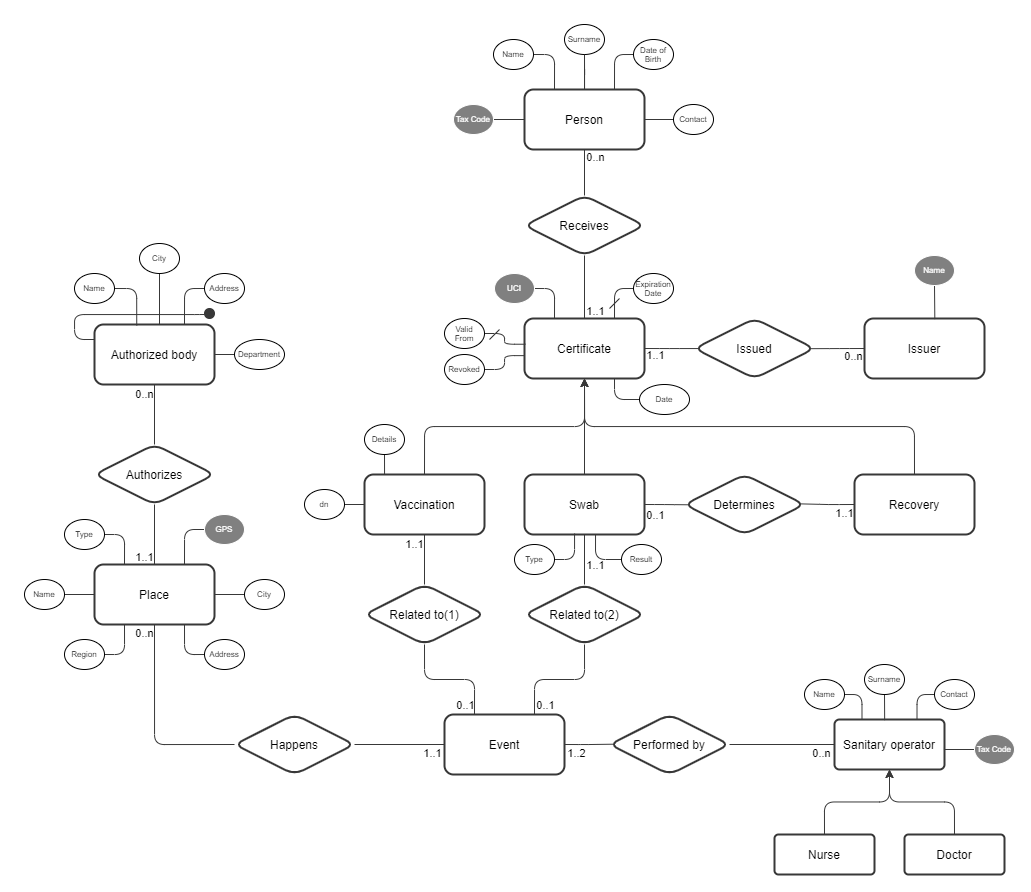
\includegraphics[scale=0.30]{er.png}
\end{figure}
\newpage

\section{Document diagram}
The designed Document diagram is shown below. Certificate and Authorized body are represented as collections of documents.

The certificate document doesn't represent an unique person but it is specific for a determined event. It can have one between Recovery, Test and Vaccination as sub-document and these last two have both Place and Sanitary operators as sub-documents which contain all the information related to the place and the doctor/nurse involved in the specific event.
\hfill\break
\\
The Recovery document has been implemented to make the recovery certificate validation easier and faster. Otherwise, doing this validation through the scan of the tests information would have been more complex due to the possibility of a person to do an unlimited amount of tests.
With this design choice the time complexity of validate a recovery certificate has been reduced.
\hfill\break
\hfill\break


\begin{center}
\includegraphics[scale=0.18]{document_diagram.png}
\end{center}
As shown above, every certificate has an unique certification number and contains all the information about the person to whom it belongs like for instance name, surname and tax code. It also has information about the period while it can be used like the validity starting date and the expiration date. 

Certificates also have a boolean value called Revoked with a False default value, which can be switched to True in case a certification has been released due to a mistake, allowing in this way the possibility to make it unusable.
\\

Vaccination, Reovery and Test contains the relevant information about the performance, like for instance the date of the event and the type of tests or vaccine.
\\

Sanitary operator and Place instead have information about when an event has happened and by whom it has been performed. This information can be useful, for instance in case of mistakes or doubts, to track down the sanitary operator or the doctor who performed the vaccination or test.

\section{Dataset description}
The Dataset has been built by making a script in Python, using some useful packages like: {\fontfamily{qcr}\selectfont random-italian-person} that automatically generates people with random attributes (this package has been modified due to our necessity); the official {\fontfamily{qcr}\selectfont PyMongo} driver for Python for the communication with the Database since it allows to make queries directly from Python.

\\
\hfill\break
It has been also used a CSV document, downloaded directly from the official Italian Government github repository, of all the vaccination centres (due to the limited scale of the to make database only some regions have been taken into consideration).

CSV files for vaccines information and authorized bodies have been built by hand due to necessity with the relevant information.


\newpage
\section{Queries and Commands}
In the following chapter all the queries and commands parameters (part of the code to substitute with desired values) will be highlighted with \textbf{\color{magenta}{magenta}} bold text. 

Some parameters information can be useful for different queries or commands so they are written here to avoid writing them multiple times:
\begin{itemize}
    \item The UCI (unique certificate identifier) is an alphanumeric string and must be in the following format: \\"01ITAXXXXXXYYYXXXYXXYXYYXYXXXXXXYXY" where X is a digit and Y is a capital letter.
    \item The tax code ("codice fiscale" in italy) is a 16 digits alphanumeric code and follow the usual italian format.
    \item Dates must be in the following format YYYY-MM-DD.
\end{itemize}
\subsection{Queries}
\subsubsection{Last expiring certificate}
The following query, given the tax code of a person, returns the date of his last expiring certificate and the UCI of such certificate. This query can be used to find out if a person
has any valid green pass or not.

\begin{lstlisting}[language=cypher, label=lst:cypher-example]

db.certificates.find(
    {
        'tax_code': "<@\textbf{\color{magenta}{tax code}}@>",
        'expiration_date' : {$exists: true}
    },
    {
        'uci': 1,
        'expiration_date': 1
    }
).sort({"expiration_date": -1}).limit(1)

\end{lstlisting}
\newpage
\subsubsection{Expiration date of certificate}
The following query, given a UCI of a certificate, returns its expiration date. This can be useful for instance for the control of certification validity for the access of public spaces. 

\begin{lstlisting}[language=cypher, label=lst:cypher-example]

db.certificates.find(
    {
        'uci': "<@\textbf{\color{magenta}{uci}}@>"
    },
    {
        "expiration_date": 1,
        "_id": 0
    }
)

\end{lstlisting}
\subsubsection{People vaccinated by a nurse}
\label{subsec:nurse-query}
This query can be used to find all the people (and therefore the related certificates with their information) that get vaccinated by a given sanitary operator in a certain period of time. It can be useful for instance in case, probably due to a mistake, a sanitary operator accidentally injects a saline solution instead of a vaccine, consequentially all the people must be tracked down and warn and their certificates must be revoked.\\
The tax code is the fiscal code of the nurse who performed the vaccination, min date and max date are the two dates which delimit the period of time.

\begin{lstlisting}[language=cypher, label=lst:cypher-example]

db.certificates.find(
    {
        "vaccination.nurse.tax_code": "<@\textbf{\color{magenta}{tax code}}@>",
        "vaccination.date": {$gte: ISODate('<@\textbf{\color{magenta}{min date}}@>'),
                             $lte: ISODate('<@\textbf{\color{magenta}{max date}}@>')}
    },
    {
        "_id": 0,
        "name": 1,
        "surname": 1,
        "tax code": 1,
        "contact": 1,
        "uci": 1,
        "vaccination.date": 1
    }
)

\end{lstlisting}
\newpage
\subsubsection{Doctor who performed an anamnesi}
This query returns the tax code of the doctor who performed the anamnesi during the last vaccination of a specific person and the related date.
It can be used for instance, in case someone die in the next days of a vaccination, to track down the doctor who performed the anamnesi to see if there is any correlation between the death and the anamnesi of the doctor. 

The tax code parameter is the fiscal code of the vaccinated person.

\begin{lstlisting}[language=cypher, label=lst:cypher-example]

db.certificates.find(
    {
        "tax_code": "<@\textbf{\color{magenta}{tax code}}@>"
    },
    {
        "vaccination.doctor.tax_code": 1,
        "vaccination.date": 1
        _id: 0
     }
).sort({"vaccination.date": -1}).limit(1)

\end{lstlisting}
\subsubsection{Covid history of a person}
The following query returns the entire Covid history (all the vaccinations and tests information) of a given person.
The tax code is the fiscal code of the person whose history you want to look for.

\begin{lstlisting}[language=cypher, label=lst:cypher-example]

db.certificates.find(
    {
        "tax code": "<@\textbf{\color{magenta}{tax code}}@>",
    },
    {
        "test": 1,
        "recovery": 1,
        "vaccination": 1,
        "_id": 0
    }
)

\end{lstlisting}
\subsubsection{Vaccination amount per period}
This query returns the amount of vaccination certificates released in a desired period. Min date and max date parameters are the two dates which delimit the period of time.

\begin{lstlisting}[language=cypher, label=lst:cypher-example]

db.certificates.countDocuments(
    {"vaccination.date": {$gte: ISODate('<@\textbf{\color{magenta}{min date}}@>'),
                          $lte: ISODate('<@\textbf{\color{magenta}{max date}}@>')}
                          }   )


\end{lstlisting}
\newpage
\subsection{Commands}
\subsubsection{New vaccination}
This query add a new vaccination (and the relevant information) for a person.

\begin{lstlisting}[language=cypher, label=lst:cypher-example]

db.certificates.insertOne({
  'name' : "<@\textbf{\color{magenta}{person name}}@>",
  'surname' : "<@\textbf{\color{magenta}{person surname}}@>",
  'dob' : "<@\textbf{\color{magenta}{person date of birth}}@>",
  'tax_code' : "<@\textbf{\color{magenta}{person tax code}}@>",
  'contact' : "<@\textbf{\color{magenta}{person mobile number}}@>",
  'emergency_name' : "<@\textbf{\color{magenta}{name of emergency contact}}@>",
  'emergency_contact' : "<@\textbf{\color{magenta}{mobile number of emergency contact}}@>",
  'uci' : "<@\textbf{\color{magenta}{certificate uci}}@>",
  'revoked' : False,
  'issuer' : "Italian Ministry of Health",
  'expiration_date': "<@\textbf{\color{magenta}{certificates expiration date}}@>"
  'valid_from' : "<@\textbf{\color{magenta}{starting validity date}}@>",
  'vaccination' : {
    'name' : "<@\textbf{\color{magenta}{vaccine name}}@>",
    'brand' : "<@\textbf{\color{magenta}{vaccine brand}}@>",
    'type' : "<@\textbf{\color{magenta}{vaccine type}}@>",
    'lot' : "<@\textbf{\color{magenta}{vaccine lot}}@>",
    'sn' : "<@\textbf{\color{magenta}{vaccine sn}}@>",
    'dn' : "<@\textbf{\color{magenta}{vaccine dn}}@>",
    'nurse' : {
      'type' : "Nurse",
      'name' : "<@\textbf{\color{magenta}{nurse name}}@>",
      'surname' : "<@\textbf{\color{magenta}{nurse surname}}@>",
      'tax_code' : "<@\textbf{\color{magenta}{nurse tax code}}@>",
      'contact' : "<@\textbf{\color{magenta}{nurse mobile number}}@>"
    },
    'doctor' : {
      'type' : "Doctor",
      'name' : "<@\textbf{\color{magenta}{doctor name}}@>",
      'surname' : "<@\textbf{\color{magenta}{doctor surname}}@>",
      'tax_code' : "<@\textbf{\color{magenta}{doctor tax code}}@>",
      'contact' : "<@\textbf{\color{magenta}{doctor mobile number}}@>"
    },
    'place': {
      'building_name' : "<@\textbf{\color{magenta}{building name}}@>",
      'type' : "<@\textbf{\color{magenta}{building type}}@>",
      'region' : "<@\textbf{\color{magenta}{building region}}@>",
      'gps' : "<@\textbf{\color{magenta}{builfing coordinates}}@>",
      'city' : "<@\textbf{\color{magenta}{building city}}@>",
      'authorized_by' : "<@\textbf{\color{magenta}{building authorized body}}@>"
    },
    'date' : "<@\textbf{\color{magenta}{vaccination date}}@>",
  }
})

\end{lstlisting}
\subsubsection{Expiration date update}
This query changes the expiration date of all the vaccination certificates related to the second dose. It can be used for instance in case of government rules changes to extend the validity of the certificates.
Days is the amount of days (integer) that will increase or decrease the validity of the certificate. Sign can only be + (for increasing) or - (for decreasing).

\begin{lstlisting}[language=cypher, label=lst:cypher-example]

db.certificates.updateMany(
    {"vaccination.dn": 2},
    [{ $set: { "vaccination.expiration_date": {
    $add: ["$vaccination.expiration_date", <@\textbf{\color{magenta}{sign}}@> 24*3600 * 1000 * <@\textbf{\color{magenta}{days}}@>]}}
    }]
)


\end{lstlisting}
\subsubsection{Revoke certificate}
The command proposed is used to revoke a certificate under a certain condition.
The utility of such command, for instance, could be to revoke all the certificates related to vaccinations performed by a given nurse in a specific day for the same motivation
explained in the nurse query in subsection \ref{subsec:nurse-query}.

\begin{lstlisting}[language=cypher, label=lst:cypher-example]

db.certificates.updateMany(
    {
        "vaccination.date": new Date("<@\textbf{\color{magenta}{YYYY-MM-DD}}@>"),
        "vaccination.nurse.tax_code": "<@\textbf{\color{magenta}{nurse tax code}}@>"
    },
    {
        "$set": {"revoked": true}
    }
)

\end{lstlisting}
\newpage
\section{Generator database}
The {\fontfamily{qcr}\selectfont"MongoDB-assignment/main.py"} file is responsible of generating a random database.
In order to correctly run the generator, it is mandatory to store the MongoDB connection string (with the correct username and password) in a .txt file named {\fontfamily{qcr}\selectfont connection-string.txt} saved in the directory {\fontfamily{qcr}\selectfont MongoDB\_assignment}.
%store the Neo4j password in {\fontfamily{qcr}\selectfont"neo4jDB-populator/password.txt"}, in this way the generator will be able to connect with the database.
\\This script exploits the following packages: {\fontfamily{qcr}\selectfont pandas, numpy, PyMongo and python-codicefiscale}.

\subsection{Place generation}
The CSV file {\fontfamily{qcr}\selectfont"datasets/locations.csv"} has been used to generate all the places related to tests and vaccinations. Due to database scale limitation the generation of places has been limited to the Lombardy region.
%This generator will create facilities data for the following cities: Rome, Milan and Naples. For each city it will create event details representing hospitals and pharmacies available in that specific town.
%For safety sake, the parameter that sets the number of public spaces to generate should be lower than 46.

\subsection{Certificate generation}
In order to consistently generate certificates information about people have been randomly generated by using our adapted version of the random italian person package. A function has been implemented in order to generate random UCI (by using a real italian format).

\subsection{Sanitary operator generation}
Sanitary operators information have been randomly generated by using our adapted version of the random italian person package.

\subsection{Authorized body generation}
The CSV file {\fontfamily{qcr}\selectfont"datasets/auth\_bodies.csv"} has been used to generate all the authorized bodies documents. Due to database scale limitation their generation has been limited to only some of them present in the Lombardy region.


\newpage
\section{Application description}
Goal of the web application {\fontfamily{qcr}\selectfont"webapp/App.py"} is to give some information about the Covid-19 history and certifications about a specific person.
The starting page of the web application is the login page where the user can use his tax code
and password.

As the main purpose of this project is not to build a full working application, the authentication procedure has not been implemented, thus it is possible to visualize the historic of a given person without
digitising any password.
\begin{center}
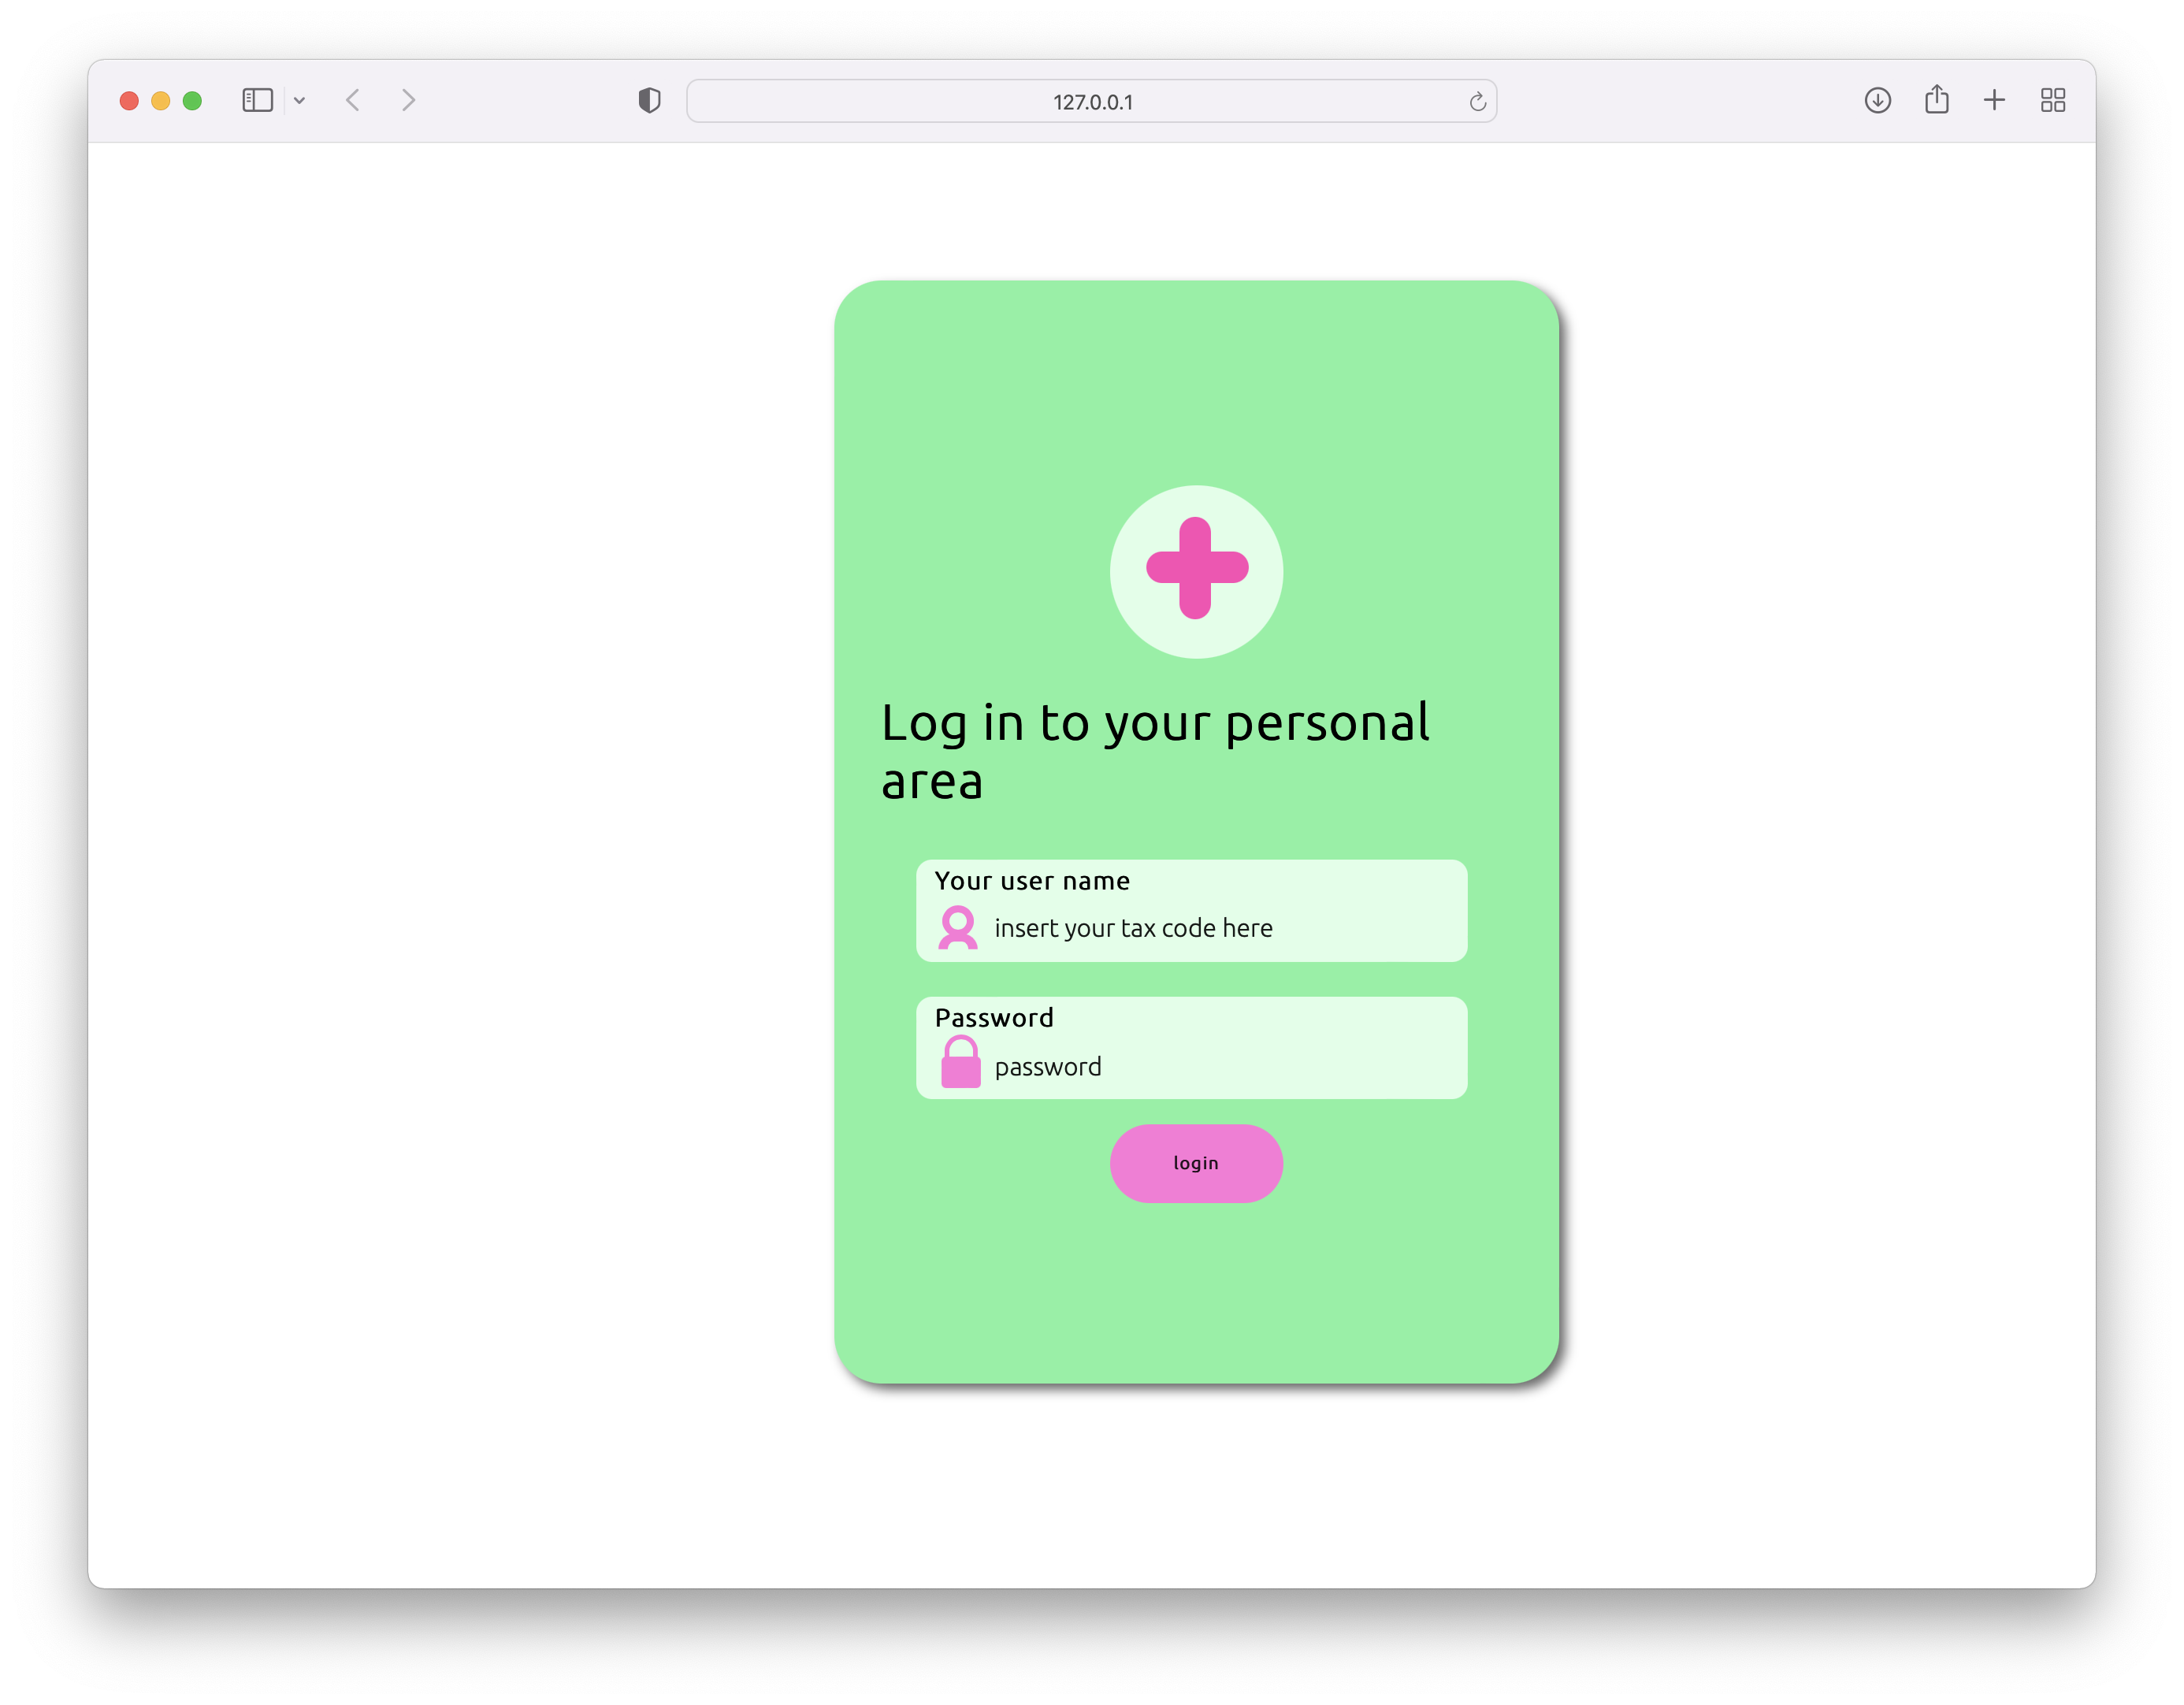
\includegraphics[scale=0.23]{login.png}
\end{center}
The user, after logged in, will be redirected to his personal area where he can:
\begin{itemize}
    \item Visualize all his/her certifications (valid or expired).
    \item Visualize his/her vaccines.
    \item Visualize all his/her tests.
\end{itemize}

\begin{figure}[h!]
  \centering
  \begin{subfigure}
    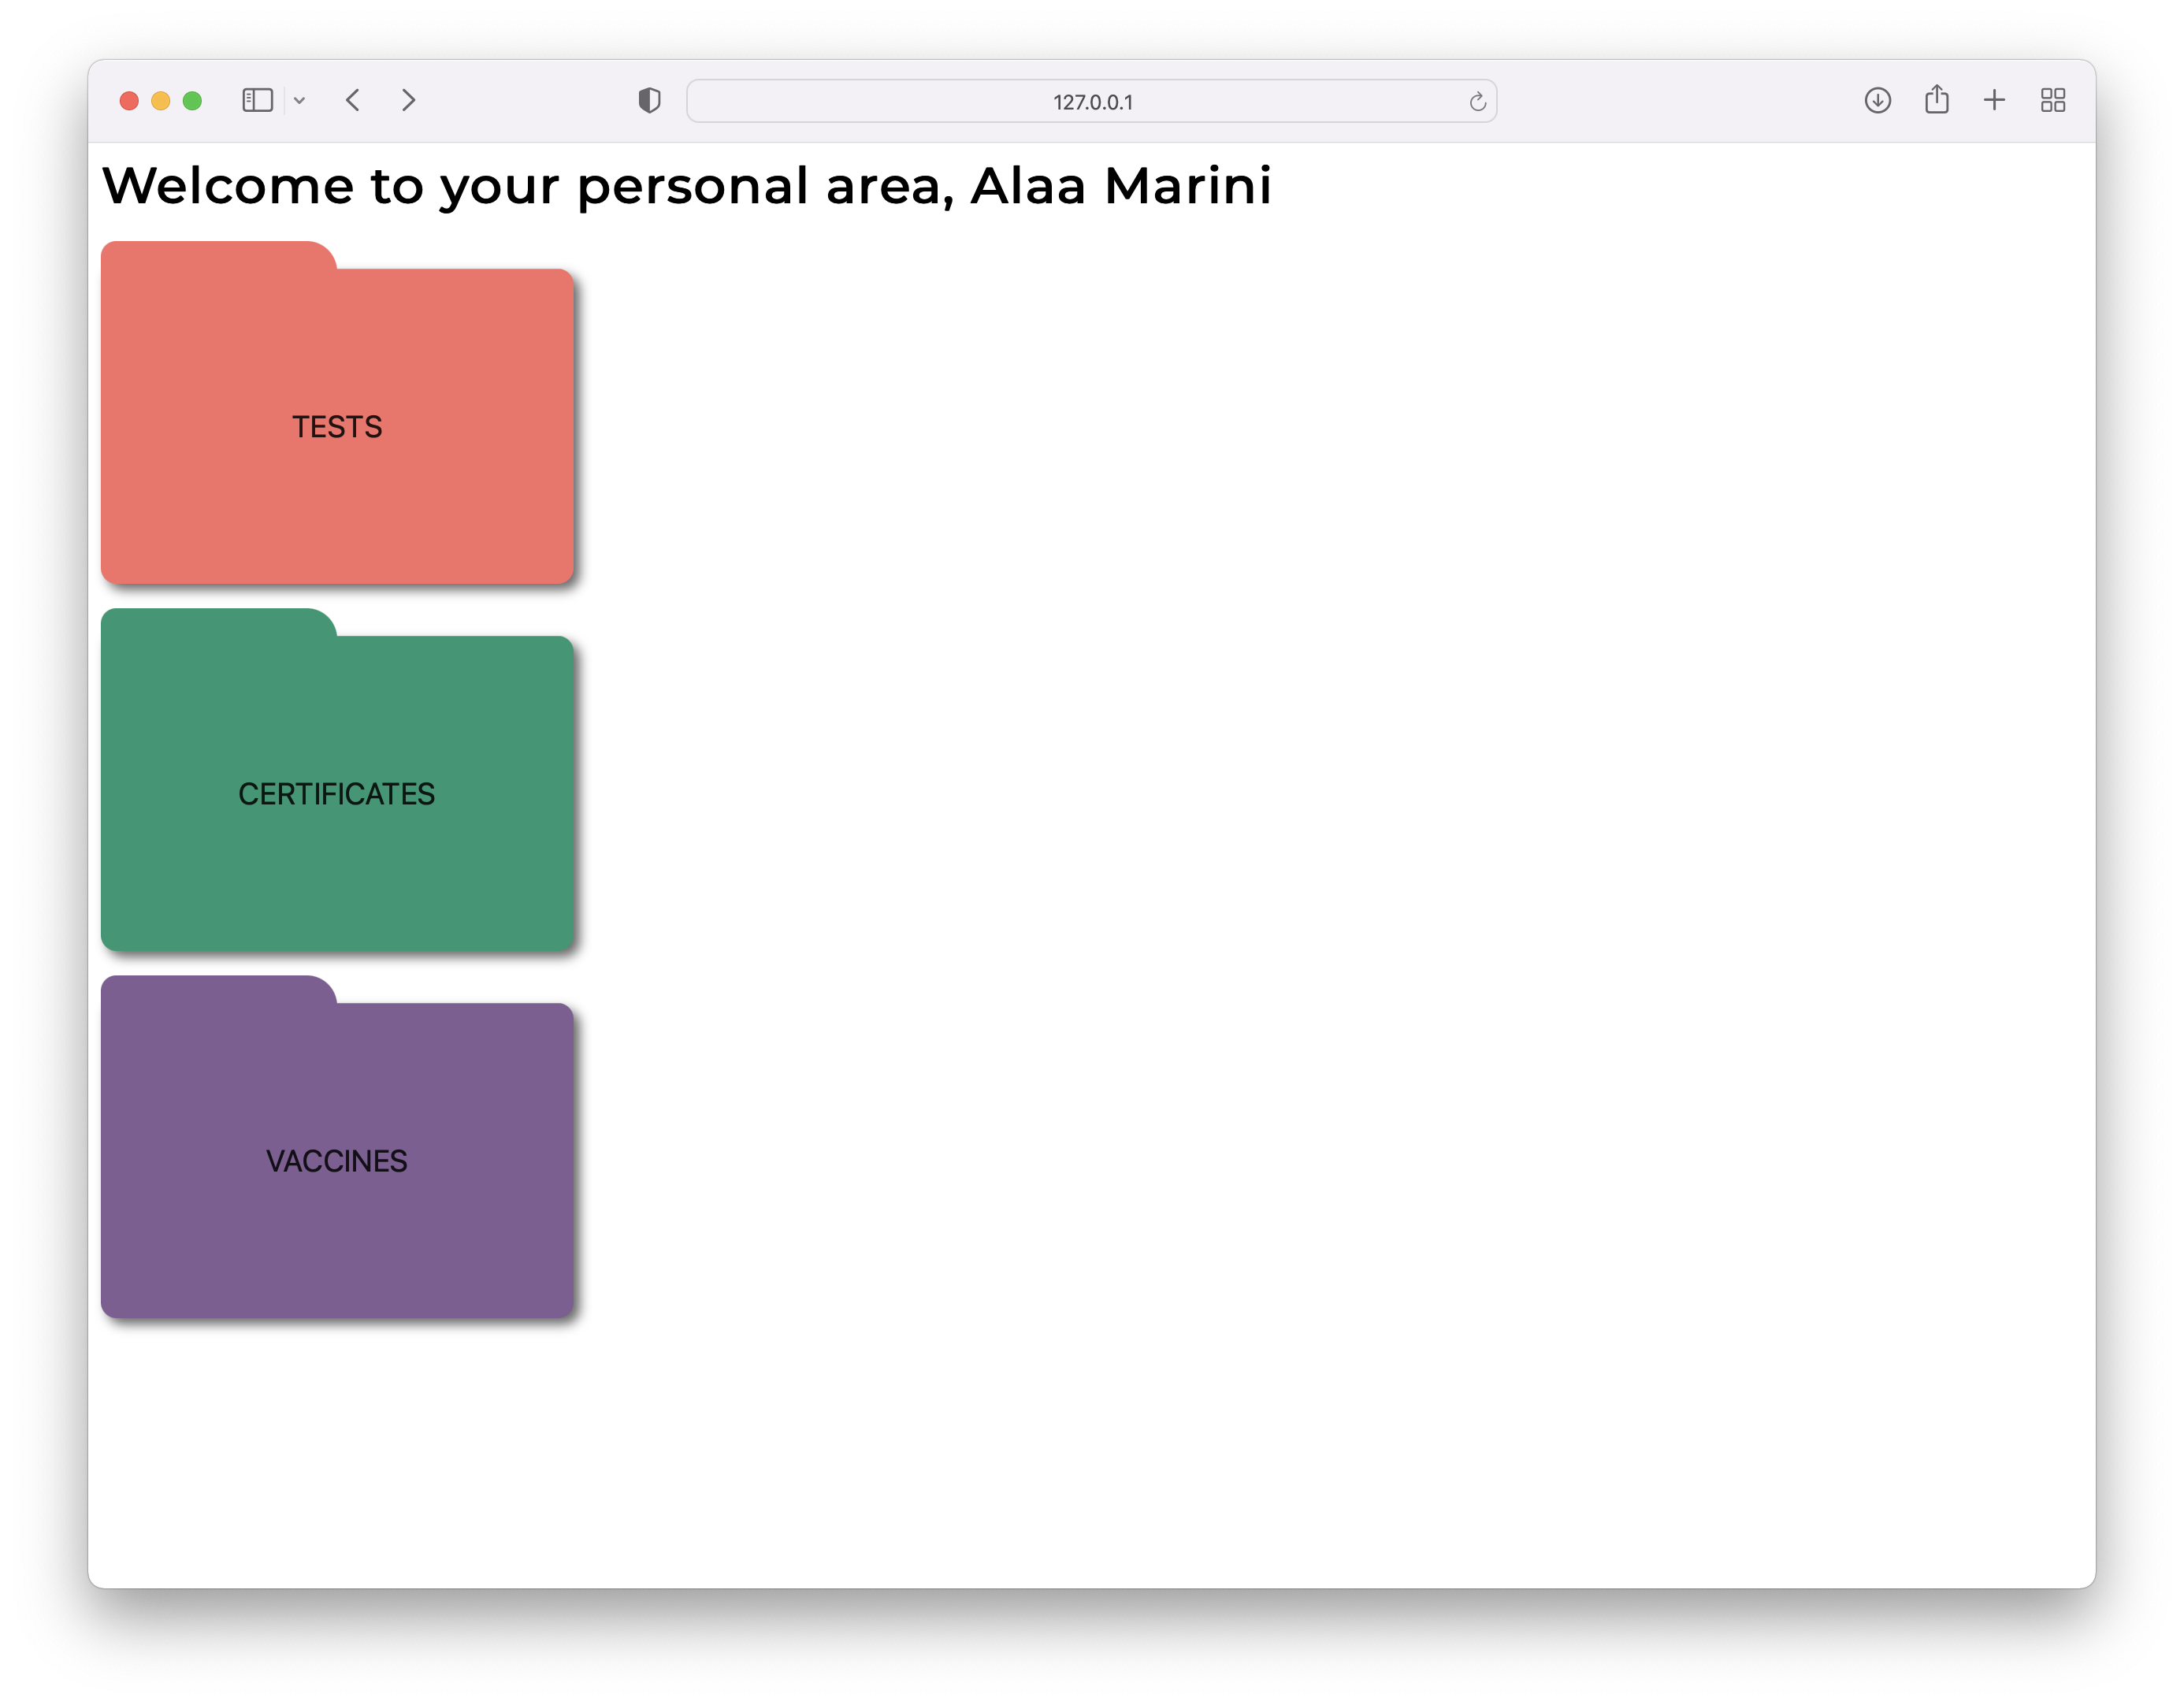
\includegraphics[scale=0.23]{home.png}
    \caption{Application displaying the personal area to the user.}
  \end{subfigure}
  \hfill \break
  \begin{subfigure}
    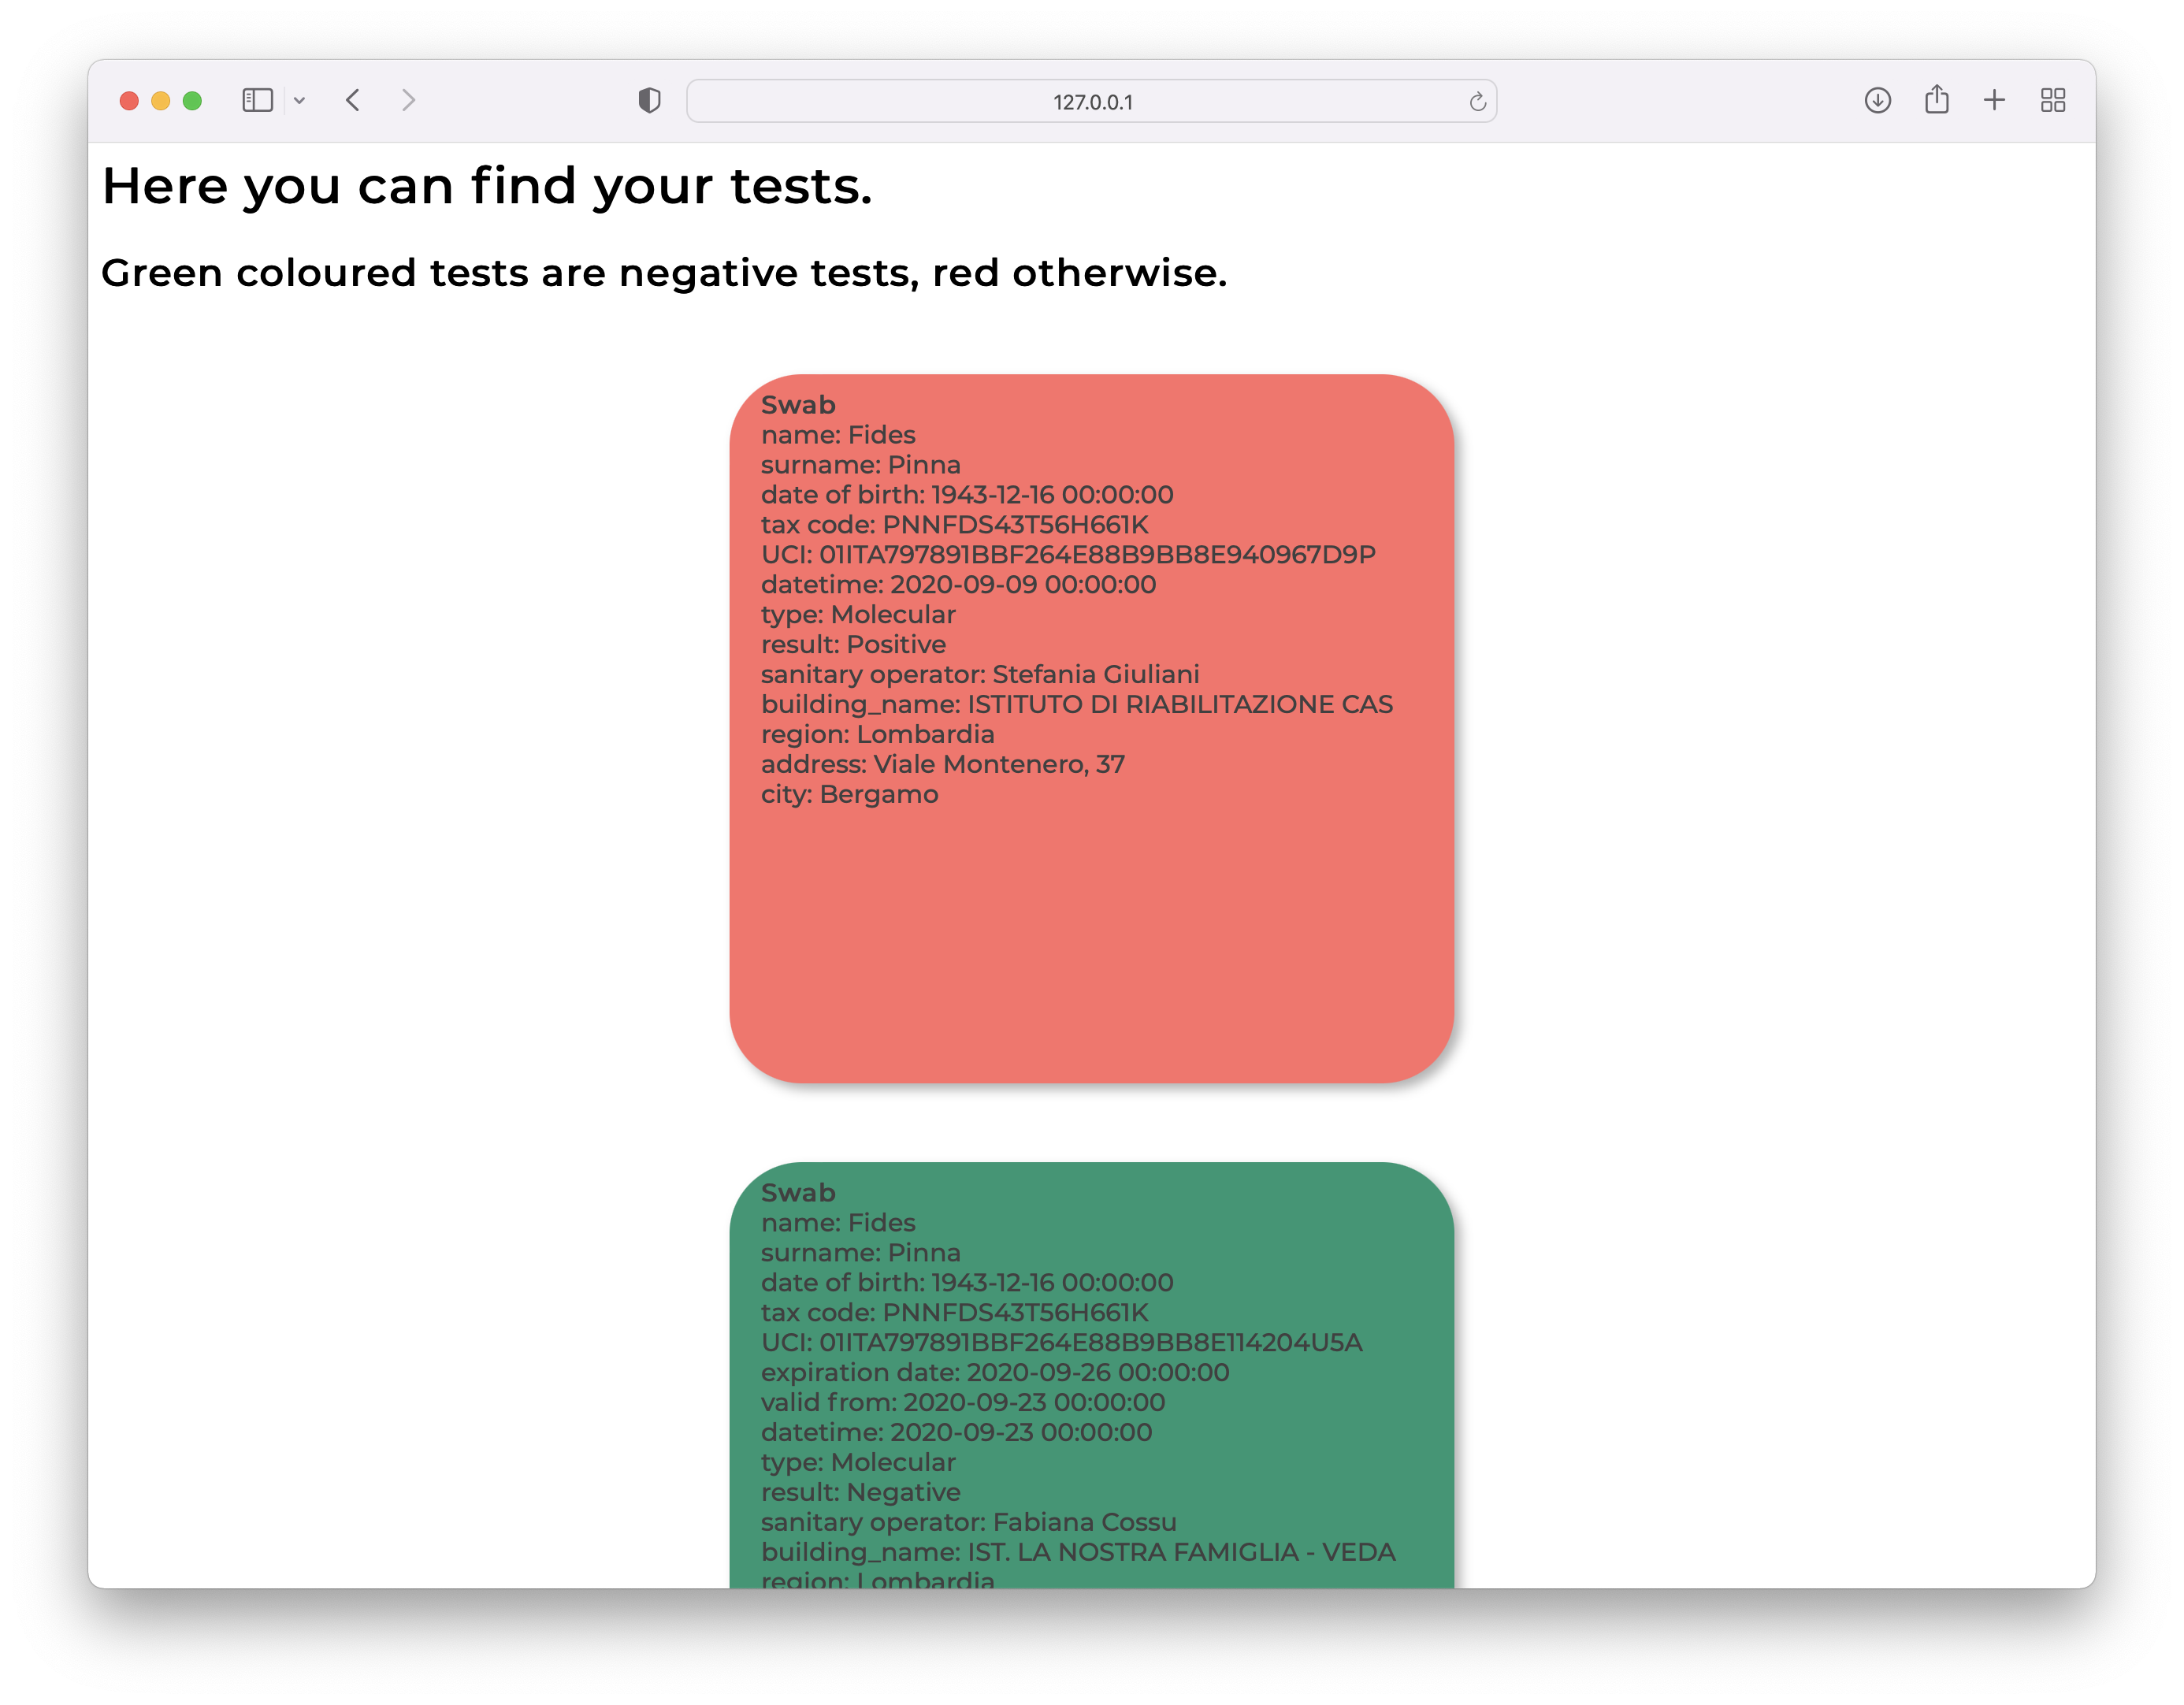
\includegraphics[scale=0.23]{tests.png}
    \caption{Application displaying the tests performed by the user. Red documents are positive tests, whereas green documents are negative tests.}
  \end{subfigure}
  \label{fig:screen_from_App}
\end{figure}

\newpage

\section{User guide}
The application is meant to work on every operating system since it is executed on a browser. As the application has been entirely developed in Python, it is not operative system dependent.
%In order to correctly run the application it is mandatory to...
%store the Neo4j password in {\fontfamily{qcr}\selectfont"neo4jDB-populator/password.txt"}, in this way the application will be able to connect with the database.
\\The user must check to have correctly installed, in the virtual environment, the following pacakges: {\fontfamily{qcr}\selectfont Flask, Flask-PyMongo, bson, PyMongo, pandas, numpy and python-codicefiscale}.
\hfill\break
\\There are two possible ways to run the demo: the first one is to connect to the following link: \href{https://c19-cert-viewer.herokuapp.com/}.

In alternative, it is possible to run locally {\fontfamily{qcr}\selectfont"webapp/App.py"} and connect to {\fontfamily{qcr}\selectfont"loacalhost:port"} where {\fontfamily{qcr}\selectfont"port"} is the port number suggested by the console.

Note that by default both {\fontfamily{qcr}\selectfont"MongoDB-assignment/main.py"} and {\fontfamily{qcr}\selectfont"MongoDB-assignment/webapp/App.py"} are connected to the same server that can be accessed by anyone, for this reason it is not mandatory to change the connection string.
\section{Conclusion}

Some interesting conclusions can be drawn from the development of this project: Document databases are, if well designed, easy to use and really scalable. Thanks to a good db structure most queries can be easily written in a compact way.

A fundamental property of MongoDB databases is the need to optimize data access, which puts the focus on query patterns. This mean that a good practice for MongoDB databases design is to consider how users will query the data and how often.

\section{References and Sources}
\begin{itemize}
    \item Random-italian-person package: https://pypi.org/project/random-italian-person
    \item PyMongo package: https://docs.mongodb.com/drivers/pymongo/
    \item Flask package: https://flask.palletsprojects.com/en/2.0.x/
    \item Italian Government repository: https://github.com/italia/covid19-opendata-vaccini
    %\item Overpass turbo API: https://wiki.openstreetmap.org/wiki/Overpass\_API
\end{itemize}



\end{document}